\section{Experiments and results}\label{chapter4}




\subsection{Dataset}
We illustrate our neural network model on given datasets: training dataset, training labels and testing dataset.
Both training and testing datasets contain multiple samples with fixed-length of features.
We also observed that the original training dataset might be applied with PCA and reduced the dimension to $60000 \times 128$ matrix.
The training label is a $60000 \times 1$ matrix.
Similarly, the testing dataset is $10000 \times 128$ matrix.
Initially we split our dataset into $50,000$ training samples and $10,000$ test samples to find the number of iteration~\texttt{n\_iter} corresponding to the maximum cross-validation accuracy as our early stopping point.
Then we use all the $60,000$ samples to build our final neural network model.

\subsection{Experiment Setup}
We apply two algorithms (\textsc{nmf} and \textsc{klnmf}) with four categories of noises (no noise, Gaussian noise, Poisson noise and Salt \& Pepper noise), which results in eight combinations in each epoch. In each epoch, we randomly select 90\% of samples to train NMF algorithms and evaluate three metrics on reconstructed images. The training will terminate when the error reaches the minimum error, or the maximum iteration is reached. The minimum error and maximum iteration are hyperparameters which we learn from iterative experiments. Our code saves the learning errors versus the number of iterations so that we could draw the plot and observe the convergence of the learning process. We increase the number of epochs and calculate the average metrics and confidence intervals.

\subsubsection{multiprocessing speed up hyperparameter tuning}
We write a shell script to run all our tests in parallel in the virtual machines on the cloud,
this helps us fully utilise our computing resources to generate the test results

\subsubsection{Hardware and software}
We use the following hardware to train our neural network model and generate the test results.

\subsubsection{Early stopping decides maximum number of iterations}

\subsection{Experiments Results}
\subsubsection{Optimal hyperparameters}

Table of results and hyperparameters with optimal and suboptimal coefficients.

\begin{figure}
	\centering
	%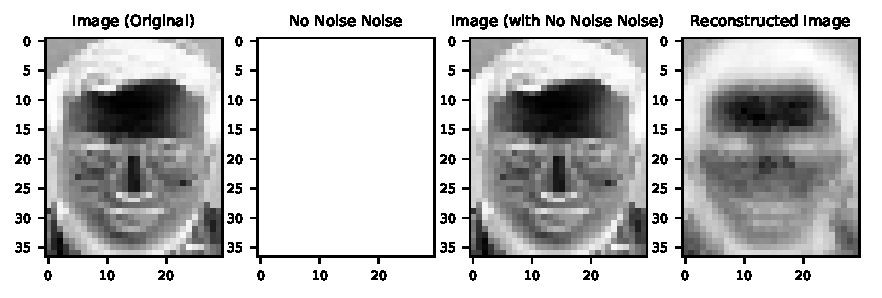
\includegraphics[scale=.9]{Result_Multiplication_KL_Divergence_No_Noise_Comparison}
\caption{Put accuracy vs iteration here with the best possible hyperparameter, and parameters without each of normalisation, dropout, momentum}\label{noisesklnmff}
\end{figure}


\begin{table}
\caption{Results and parameters of the best four setups.}
{\footnotesize
% \label{tab:ci}\begin{tabular}{l|lll}
%  \hline
% \texttt{ORL} dataset & \textsc{rre} & \textsc{acc} & \textsc{nmi}\tabularnewline
%  \hline
% \textsc{nmf} no noise & 0.1583 (0.1581, 0.1584) & 0.7364 (0.731, 0.742) & 0.8536 (0.8506, 0.8567)\tabularnewline
% \hline
% \end{tabular}}
\centering
\begin{tabular}{@{}llllll@{}}
\toprule
Experiment                & Test 1  & Test 2           & Test 3           & Test 4  & Test 5  \\ \midrule
Runtime(mins)             & 2.3     & 2.7              & 3.6              & 17.2    & 10.8    \\
Accurarcy                 & 89.9\%  & 89.7\%           & 89.8\%           & 90.0\%  & 89.3\%  \\
Initialisation            & Xavier  & Uniform$(-1,1)$ & Uniform$(-1,1)$ & Xavier  & Xavier  \\
Batch size                & 1500    & 1500             & 1500             & 1500    & 1500    \\
Hidden layer nodes        & 160     & 150              & 150              & 900     & 160     \\
Activation function       & $\tanh$ & $\tanh$          & $\tanh$          & $\tanh$ & sigmoid \\
Weight decay rate         & 0.0007  & 0.0007           & 0.0007           & 0.007   & 0.007   \\
Momentum rate             & 0.9     & 0.9              & 0.92             & 0.9     & 0.9     \\
Dropout rate              & 0.95    & 1.0              & 1.0              & 0.5     & 0.95    \\
Learning rate             & 0.11    & 0.05             & 0.05             & 0.11    & 0.11    \\
Early stopping iterations & 44      & 54               & 66               & 158     & 282     \\ \bottomrule
\end{tabular}
%\csvautobooktabular{resource/table1.csv}
}
\end{table}

\begin{table}
\caption{Results and parameters of different setups for 89.87 results.}
{\footnotesize \centering
\begin{tabular}{@{}lrrrrr@{}}
\toprule
Experiment                & Test 1  & Mini-Batch & Weight decay & Momentum & Drop out 50\% \\ \midrule
Runtime(minutes)          & 2.3     & 0.5        & 8.6          & 0.8      & 7.6           \\
Accurarcy                 & 89.9\%  & 85.5\%     & 89.4\%       & 88.6\%   & 87.5\%        \\
Initialisation            & Xavier  & Xavier     & Xavier       & Xavier   & Xavier        \\
Batch size                & 1500    & 1500       & 1500         & 1500     & 60000         \\
Hidden layer nodes        & 160     & 160        & 160          & 160      & 160           \\
Activation function       & $\tanh$ & $\tanh$    & $\tanh$      & $\tanh$  & $\tanh$       \\
Weight decay rate         & 0.0007  & 0.0007     & 0.0007       & 0        & 0.007         \\
Momentum rate             & 0.9     & 0.9        & 0            & 0.9      & 0.9           \\
Dropout rate              & 0.95    & 0.5        & 0.95         & 0.95     & 0.95          \\
Learning rate             & 0.11    & 0.11       & 0.11         & 0.11     & 0.11          \\
Early stopping iterations & 44      & 9          & 198          & 16       & 177           \\ \bottomrule
\end{tabular}
}
\end{table}

\begin{figure}
    \center{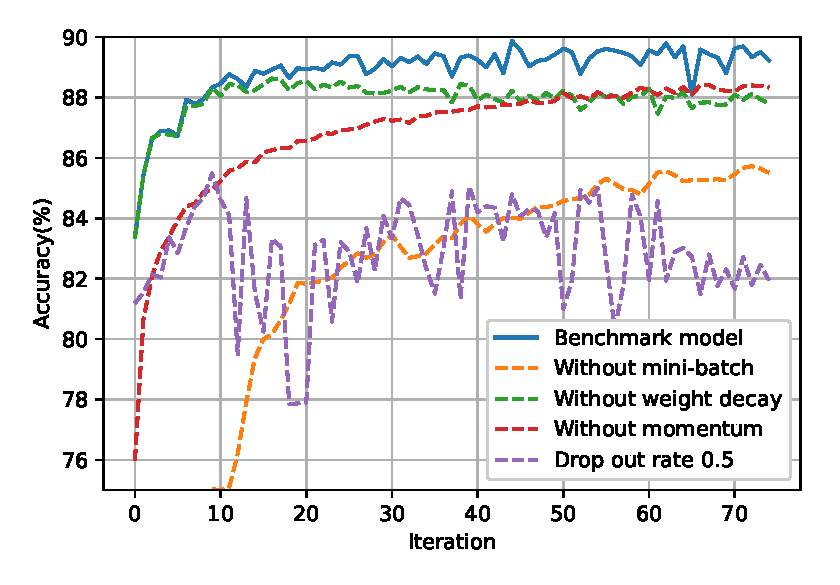
\includegraphics
    {resource/acc.eps}}
    \caption{\label{fig:my-label}Results and parameters of different setups for 89.87 results.}
\end{figure}

\begin{figure}
    \center{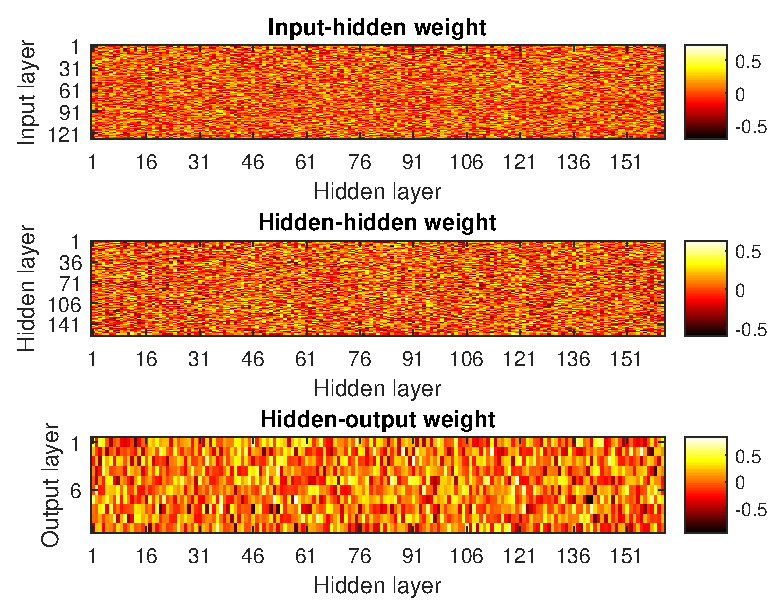
\includegraphics
    {resource/figure2.eps}}
    \caption{\label{fig:my-label}Weight Matrix on multiple layers.}
\end{figure}


\subsection{Experiments Results}
\subsubsection{Vectorisation dramatically improves the speed of training}
\subsubsection{Batch normalisation significantly improves the accuracy}
\subsubsection{Weight decaying prevents overfitting}
\subsubsection{dropout does not help here}
